%%% LaTeX Template: Article/Thesis/etc. with colored headings and special fonts
%%%
%%% Source: http://www.howtotex.com/
%%% Feel free to distribute this template, but please keep to referal to http://www.howtotex.com/ here.
%%% February 2011

%%%%% Preamble
\documentclass[10pt,a4paper]{article}

\usepackage[T1]{fontenc}

\usepackage[utf8]{inputenc}							% Input encoding
\usepackage{amsmath}
\usepackage{amssymb}									% Math
\usepackage{graphicx}

\usepackage{amsthm}

\usepackage{url}

\usepackage{tcolorbox}
\tcbuselibrary{theorems}

%%%%% Definitions

\title{Bayesian Task Description}
\author{Sarah Lutteropp}

\newtheorem{definition}{Definition}
\newtheorem{example}{Example}
\newtheorem{theorem}{Theorem}

\begin{document}
\maketitle

\begin{abstract}
The following document sums up the tasks for the Bayesian implementation of the new PTP heuristic.
\end{abstract}

\section{The Problem}
The current new PTP heuristic tends to oversplit the taxa into too many species. We believe that this is a fundamental problem with the currently used maximum likelihood model.

\section{The Solution}
We will use a prior for the number of species in the tree. Since we do not know the prior distribution, we will use a hyperprior approach for that.

\paragraph{Candidate Distributions for the Prior}
\begin{itemize}
\item Negative binomial distribution (since it is the discrete analogue of the gamma distribution)
\item Binomial distribution
\item Dirichlet

\item Beta distribution
\item Uniform distribution
\end{itemize}

\textcolor{red}{\textbf{Still unclear to me: Why should we use this distribution? Does it make any sense? It describes the number of trials needed until you have a given number of successes in a Bernoulli experiment \ldots What is the connection to the number of species?!}}

\paragraph{Candidate Distributions for the Hyperprior}
We will try the following distributions for $\alpha$:
\begin{itemize}
	\item Uniform
	\item Exponential
\end{itemize}

\textcolor{red}{\textbf{Still unclear to me: Which values will we use for the parameter of the hyperprior distribution in case of exponential?}}

\section{Hyperprior Approach}
The likelihood of a given delimitation is multiplied with the likelihood for the number of delimited species (will be implemented by adding the loglikelihood score of the number of species to the old loglikelihood score).


\begin{itemize}
	\item Draw an $\alpha$: Like in MCMC methods, use the hastings ratio: Always accept a better value for alpha, accept a worse value for alpha with the probability of the likelihood ratio.
	\textcolor{red}{\textbf{Still unclear to me: Does this make sense? Do we know what a ``better'' alpha is?}}
	\item Apply the heuristic for this specific alpha
	\item Count the number of speciation events gotten by the heuristic for different alphas $\Rightarrow$ Gives a posterior probability for the number of species
	\item Run it once more with those relative frequencies gotten
\end{itemize}

\paragraph{Expected Output}
\begin{itemize}
\item Relative frequencies of the number of speciation events in the results from the heuristics
\item Delimitation obtained by the heuristic with the distribution of species numbers gotten by the relative frequencies
\item Delimitation that gave the best overall likelihood score during the runs 
\end{itemize}

\section{Evaluation of the Results}
We will decide for the approach that led to approximately the same number of species as our simulated ``true'' data.

\textcolor{red}{\textbf{How do we avoid overfitting?}}

\section{Support Values}
Biologists are happy about support values for each speciation event. We need to try these two approaches:
\begin{itemize}
	\item exact matching
	\item subset matching (will lead to higher support values)
\end{itemize}

\begin{figure}[h!]
\centering
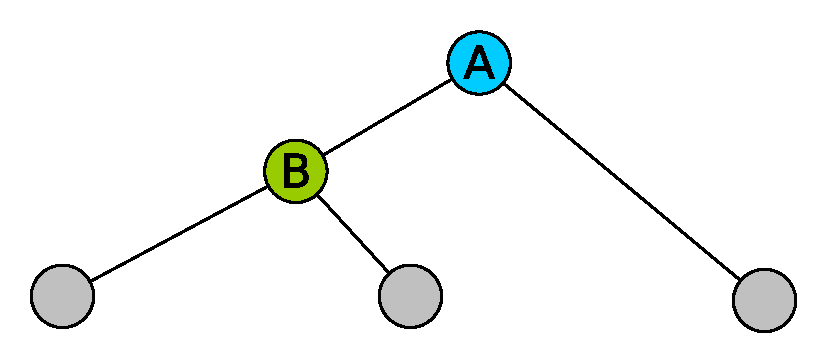
\includegraphics[scale=0.2]{images/support_tree.pdf}
\caption{Difference between exact matching and subset matching: Does the choice of MRCA $B$ also support the MRCA $A$ (or vice versa)?}
\end{figure}

\end{document}
